\documentclass{beamer}
\mode<presentation>
\usepackage{amsmath}
\usepackage{amssymb}
%\usepackage{advdate}
\usepackage{graphicx}
\graphicspath{{./figs/}}
\usepackage{adjustbox}
\usepackage{subcaption}
\usepackage{enumitem}
\usepackage{multicol}
\usepackage{mathtools}
\usepackage{listings}
\usepackage{url}
\def\UrlBreaks{\do\/\do-}
\usetheme{Boadilla}
\usecolortheme{lily}
\setbeamertemplate{footline}
{
  \leavevmode%
  \hbox{%
  \begin{beamercolorbox}[wd=\paperwidth,ht=2.25ex,dp=1ex,right]{author in head/foot}%
    \insertframenumber{} / \inserttotalframenumber\hspace*{2ex} 
  \end{beamercolorbox}}%
  \vskip0pt%
}
\setbeamertemplate{navigation symbols}{}

\providecommand{\nCr}[2]{\,^{#1}C_{#2}} % nCr
\providecommand{\nPr}[2]{\,^{#1}P_{#2}} % nPr
\providecommand{\mbf}{\mathbf}
\providecommand{\pr}[1]{\ensuremath{\Pr\left(#1\right)}}
\providecommand{\qfunc}[1]{\ensuremath{Q\left(#1\right)}}
\providecommand{\sbrak}[1]{\ensuremath{{}\left[#1\right]}}
\providecommand{\lsbrak}[1]{\ensuremath{{}\left[#1\right.}}
\providecommand{\rsbrak}[1]{\ensuremath{{}\left.#1\right]}}
\providecommand{\brak}[1]{\ensuremath{\left(#1\right)}}
\providecommand{\lbrak}[1]{\ensuremath{\left(#1\right.}}
\providecommand{\rbrak}[1]{\ensuremath{\left.#1\right)}}
\providecommand{\cbrak}[1]{\ensuremath{\left\{#1\right\}}}
\providecommand{\lcbrak}[1]{\ensuremath{\left\{#1\right.}}
\providecommand{\rcbrak}[1]{\ensuremath{\left.#1\right\}}}
\theoremstyle{remark}
\newtheorem{rem}{Remark}
\newcommand{\sgn}{\mathop{\mathrm{sgn}}}
\providecommand{\abs}[1]{\left\vert#1\right\vert}
\providecommand{\res}[1]{\Res\displaylimits_{#1}} 
\providecommand{\norm}[1]{\lVert#1\rVert}
\providecommand{\mtx}[1]{\mathbf{#1}}
\providecommand{\mean}[1]{E\left[ #1 \right]}
\providecommand{\fourier}{\overset{\mathcal{F}}{ \rightleftharpoons}}
%\providecommand{\hilbert}{\overset{\mathcal{H}}{ \rightleftharpoons}}
\providecommand{\system}[1]{\overset{\mathcal{#1}}{ \longleftrightarrow}}
%\providecommand{\system}{\overset{\mathcal{H}}{ \longleftrightarrow}}
	%\newcommand{\solution}[2]{\textbf{Solution:}{#1}}
%\newcommand{\solution}{\noindent \textbf{Solution: }}
\providecommand{\dec}[2]{\ensuremath{\overset{#1}{\underset{#2}{\gtrless}}}}
\newcommand{\myvec}[1]{\ensuremath{\begin{pmatrix}#1\end{pmatrix}}}
\let\vec\mathbf

\lstset{
%language=C,
frame=single, 
breaklines=true,
columns=fullflexible
}

\numberwithin{equation}{section}

\title{2.2.14}
\author{ai25btech11022 - Narshitha}
% \maketitle
% \newpage
% \bigskip
\begin{document}
{\let\newpage\relax\maketitle}
\renewcommand{\thefigure}{\theenumi}
\renewcommand{\thetable}{\theenumi} 
\textbf{Question}:\\The angle between the line \\
\begin{align}
\vec{r}=\brak{5\hat{i}-\hat{j}-4\hat{k}}+\lambda\brak{2\hat{i}-\hat{j}+\hat{k}}
\end{align}
and the plane 
\begin{align}
   \vec{r}.\brak{3\hat{i}-4\hat{j}-\hat{k}}+5=0
\end{align}
is\\
\textbf{Solution}:
The given line can be expressed in the form as \\
\begin{align}
    \vec{r}=\myvec{5\\-1\\-4}+\lambda\myvec{2\\-1\\1}
\end{align}
Hence the vector direction of this line is
\begin{align}
    \myvec{2\\-1\\1}
\end{align}
the normal vector of the given plane is
\begin{align}
    \myvec{3\\-4\\-1}
\end{align}
by the formula
\begin{align}
    \cos\theta=\frac{\vec{a}^T\vec{b}}{\|\vec{a}\|\|\vec{b}\|}
\end{align}
Thus the cosine of the angle between the two is
\begin{align}
\frac{3\sqrt{3}}{2\sqrt{13}}
\end{align}
which is sine of the angle between the plane and the line.\\
$\therefore$ The angle between the line and plane is $\sin^{-1}\frac{3\sqrt{3}}{2\sqrt{13}}$

\frametitle{Graphical Representation}
\begin{center}
    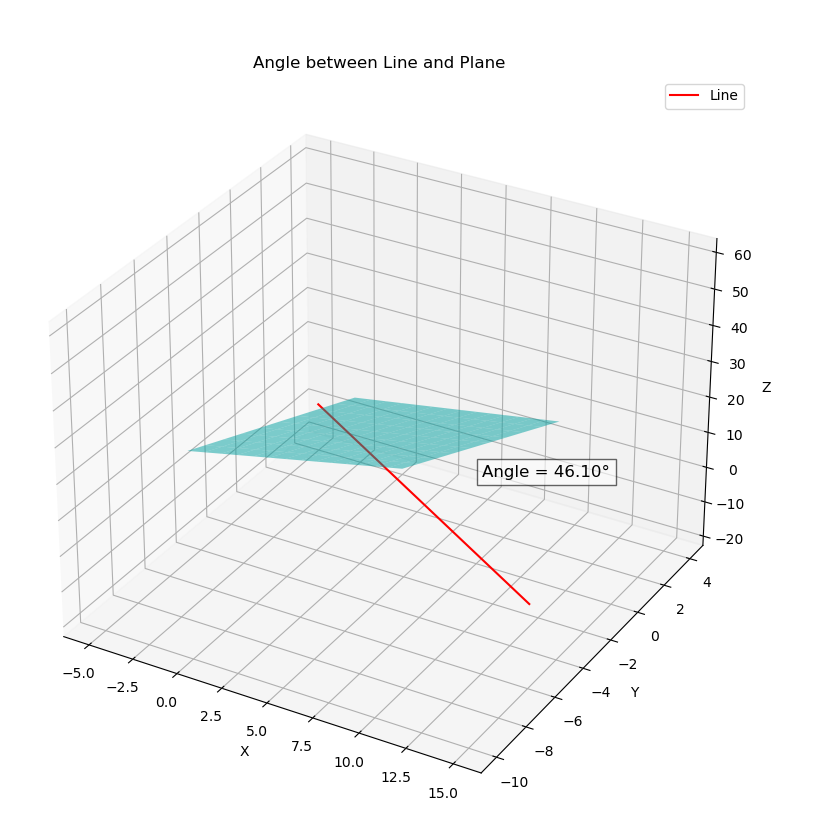
\includegraphics[width=0.7\linewidth]{figs/fig1.png}
\end{center}
    

\end{document}

